\documentclass[11pt]{article}

\usepackage[a4paper,margin=2.3cm]{geometry}
\usepackage{graphicx}
\usepackage{booktabs}
\usepackage{amsmath}
\usepackage{hyperref}
\usepackage{xcolor}
\usepackage{caption}
\usepackage{titlesec}
\usepackage{setspace}

\hypersetup{colorlinks=true, linkcolor=blue!45!black, urlcolor=blue!45!black, citecolor=blue!45!black}
\captionsetup{font=small, labelfont=bf}
\titleformat{\section}{\normalfont\large\bfseries}{}{0em}{}
\titleformat{\subsection}{\normalfont\bfseries}{}{0em}{}
\onehalfspacing

\title{\textbf{Supporting Information}\\[0.3em]
Probabilistic dengue and chikungunya forecasting in Brazil:\\
metric-dependent model rankings, regime-shift fragility, and conformal ensembles}
\date{}

\begin{document}
\maketitle
\vspace{-2em}

\noindent This document provides the scoring definitions (S1), full model configurations (S2), the
conformal recalibration and ensemble-composition robustness analysis (S3), normalized WIS by season
(S4), the EPIFORGE 2020 reporting checklist (S5), exploratory data analysis (S6), the
reproducibility statement (S7), per-state model performance (S8), calibration by percentile of the
predictive distribution (S9), and a glossary of the technical terms used in the main text (S10).
All numbers correspond to the committed backtest and are reproducible from the released pipeline.

\section*{S1 Text. Scoring}
Forecasts are submitted as the nine quantiles $\tau \in \{0.025, 0.05, 0.10, 0.25, 0.50, 0.75, 0.90,
0.95, 0.975\}$ per state and week, which define the median and the four central prediction intervals
at nominal levels 50, 80, 90, and 95 percent. The weighted interval score is
\[
\begin{aligned}
\mathrm{WIS}(F,y)&=\frac{1}{K+\tfrac12}\Big[\tfrac12\,|y-m| + \sum_{k=1}^{K}\frac{\alpha_k}{2}\,
\mathrm{IS}_{\alpha_k}(\ell_k,u_k,y)\Big],\\[0.35em]
\mathrm{IS}_{\alpha}(\ell,u,y)&=(u-\ell)+\tfrac{2}{\alpha}(\ell-y)\mathbf{1}\{y<\ell\}
+\tfrac{2}{\alpha}(y-u)\mathbf{1}\{y>u\},
\end{aligned}
\]
with $m$ the predictive median, $K=4$ central intervals, and $\alpha_k = 1 - L_k/100$. This equals the
mean pinball loss over the nine quantiles up to the constant weighting, the exact discrete
approximation to the continuous ranked probability score. We verified our implementation against the
challenge platform's own scorer to machine precision on a shared set of forecasts, and against a
hand-computed toy case that caught an early normalization error (division by $9$ rather than
$K+\tfrac12 = 4.5$): for median $m=10$, a 50 percent interval $[6,14]$, a 90 percent interval
$[2,20]$, and $y=15$, the median term is $0.5|15-10|=2.5$; $\mathrm{IS}_{0.5}=(14-6)+\tfrac{2}{0.5}
(15-14)=12$, weighted by $\alpha/2=0.25$ to $3$; $\mathrm{IS}_{0.1}=(20-2)=18$ (not exceeded, so no
penalty term), weighted by $0.05$ to $0.9$; giving $\mathrm{WIS}=(2.5+3+0.9)/(2+0.5)=2.56$ for this
$K=2$ toy case (the full score uses all four official intervals, $K=4$). This score decomposes
exactly into three non-negative components: a dispersion term (the interval-width contribution,
present even when the median is exactly correct), an under-prediction penalty (positive only when
$y$ exceeds the interval's upper bound), and an over-prediction penalty (positive only when $y$ falls
below the lower bound); their sum is bit-for-bit equal to WIS by construction, which we also test.
Alongside mean WIS we report: empirical interval coverage; that dispersion/under-prediction/
over-prediction decomposition of WIS; a per-unit relative WIS
that scores each state-season-horizon against the naive baseline and takes a geometric mean, which
weights every unit equally; and the normalized WIS, the sum of WIS divided by the sum of observed
cases, which is the challenge's headline metric and is scale-free across regions.

\section*{S2 Text. Model configurations}
\textbf{Features (gradient boosting).} Both gradient-boosting implementations evaluated in the main
text, LightGBM and
XGBoost, are fit on the identical synthetic-origin panel that
expands each fold into many weekly origins crossed with forecast horizons 1 to 67 weeks, with
origin-anchored features computed only from the cutoff-filtered history:
\begin{itemize}
\item \emph{Autoregressive:} log-incidence lags at 1, 2, 3, 4, 8, and 52 weeks; rolling mean over 4
and 8 weeks; rolling standard deviation over 4 weeks; rolling maximum over 12 weeks.
\item \emph{Seasonality:} target epidemiological week; first and second sine and cosine harmonics; a
target-relative seasonal anchor equal to the most recent same-target-epiweek incidence at or before
the origin.
\item \emph{Observed climate (four-week means at the origin):} temperature, precipitation, and
relative humidity, plus a temperature anomaly against each state's same-epiweek climatology.
\item \emph{Seasonal climate forecast:} the seasonal forecast of temperature, humidity, and
precipitation for the target month, merged leakage-safely so that only forecasts issued at or before
the origin are used.
\item \emph{Ocean oscillation indices:} El Ni\~no--Southern Oscillation, Indian Ocean Dipole, and
Pacific Decadal Oscillation, each at lags 0, 4, 8, 12, 26, and 52 weeks.
\item \emph{Static:} log population; population-weighted K\"oppen climate-zone fractions; biome
fractions; forecast horizon in weeks.
\end{itemize}

\noindent\textbf{Hyperparameters (S1 Table).} Table~\ref{tab:hparams} lists the frozen configuration
of each model. These were chosen a priori as conservative defaults. A separate search that preferred a
deeper boosted configuration (num\_leaves 63, max\_depth 7) improved an internal time-block holdout by
about 5 percent but worsened the true backtest, and was not adopted (main text
the main text, negative results).

\begin{table}[t]
\centering\small
\caption{\textbf{S1 Table. Frozen model configurations.}}
\label{tab:hparams}
\begin{tabular}{@{}p{0.22\textwidth}p{0.7\textwidth}@{}}
\toprule
\textbf{Model} & \textbf{Configuration} \\
\midrule
LightGBM (per quantile) & objective: quantile at each of the nine levels; num\_leaves 31; max\_depth 5;
learning\_rate 0.05; 400 boosting rounds; feature\_fraction 0.8; bagging\_fraction 0.8; bagging\_freq 1;
seed 42; deterministic. Intervals calibrated by conformalized quantile regression on a trailing
78-week window. Used for the chikungunya-state track; superseded by XGBoost below for the dengue
ensemble. \\
\addlinespace
XGBoost (multi-quantile, chosen for dengue) & objective: \texttt{reg:quantileerror} with
\texttt{quantile\_alpha} set to all nine levels jointly, \texttt{multi\_strategy=}
\texttt{multi\_output\_tree} (one booster covers all quantiles); \texttt{tree\_method=hist};
max\_depth 5; min\_child\_weight 30; learning\_rate 0.05; 400 boosting rounds; subsample 0.8;
colsample\_bytree 0.8; seed 42. Same feature set and CQR calibration scheme as LightGBM above. \\
\addlinespace
GRU deep ensemble & input sequence length 104 weeks; single-layer GRU encoder, hidden size 48, shared
across all 26 states; per-state embedding of dimension 8; decoder is a two-layer perceptron with
hidden size 64, ReLU, and dropout 0.1; negative-binomial output head; quantiles analytic from the
predictive distribution; deep ensemble of 5 independently seeded runs pooled by quantile averaging;
40 epochs, Adam, learning rate $10^{-3}$. \\
\addlinespace
Semi-mechanistic & 800 bootstrap resamples of whole historical season trajectories; season length 53
weeks; negative-binomial observation model; a local reimplementation of Richards-curve
epidemic-scanner fits. \\
\addlinespace
Ensembles & per-quantile median (Vincentization) of the climatological, gradient-boosted, and
deep-learning models; and inverse-WIS weighting tuned only on the designated tuning season. \\
\bottomrule
\end{tabular}
\end{table}

\section*{S3 Text. Conformal recalibration and ensemble composition}
\textbf{Conformal recalibration.} For each central interval level $L$ with bounds $[\ell_L,u_L]$ and
median $m$, and for each calibration unit, the multiplicative factor needed to just cover the
observation is $r=(y-m)/(u_L-m)$ when $y>m$ and $r=(m-y)/(m-\ell_L)$ when $y<m$, and $0$ otherwise. The
widening factor $s_L$ is the $L/100$ empirical quantile of $r$ over the tuning season, so that widening
the interval about the median by $s_L$ yields approximately $L$ percent empirical coverage. The
estimated factors are $s_{50}=1.08$, $s_{80}=1.04$, $s_{90}=1.19$, and $s_{95}=1.86$. They are gentle
and concentrate on the outer tails, which is why the recalibration protects against catastrophic
under-prediction in the outbreak season at small cost in ordinary seasons. Recalibrating the ensemble
output outperforms recalibrating any single member, because the per-quantile median across members
otherwise dilutes a member's widening (recalibrating the deep-learning member alone yields mean WIS
1273 versus 1162 for the ensemble-output recalibration).

\noindent\textbf{Member-composition robustness (S2 Table).} Table~\ref{tab:sweep} scores all eleven
two-, three-, and four-member subsets of the four candidate models under the same conformal
recalibration. The chosen three-member ensemble is close to the
best composition by the headline normalized WIS, and no subset is better on both the all-season and the
ordinary-season metric. The subset that appears best by all-season mean WIS and normalized WIS
(climatological plus mechanistic, 1141 and 0.551) is the worst of the strong subsets on ordinary
seasons (normalized WIS 0.455 versus 0.375), because it wins only by handling the 2024 outlier and
drops the two machine-learning models that carry the ordinary-season signal -- the composition-level
analogue of the metric-disagreement finding. It is also, by construction, an unreliable way to choose
a composition: evaluating candidate subsets on the very seasons being reported invites exactly the
overfitting the tuning-fold discipline exists to prevent. Scoring each candidate on fold 1 alone
(the only fold this project's own discipline permits for such a decision) instead of on the full
four-season table exposes this directly: the climatological-plus-mechanistic subset that looks best
on the reported seasons is in fact one of the worst by that fold-1 criterion (normalized WIS 0.390,
against 0.306 for the chosen composition), a within-study demonstration of why ensemble composition
should be fixed by the tuning fold and not by inspecting the headline table.

One subset does edge the chosen composition on fold 1: XGBoost plus GRU, at 0.282 against 0.306. We
did not adopt it, for the same reason the rest of this analysis gives. The composition was fixed in
advance by structure, one baseline plus one gradient-boosted plus one deep model, rather than
selected from this table, and a margin of 0.024 picked out of eleven candidates scored on a single
fold is the search artifact this discipline exists to discount, not evidence against a pre-specified
choice. That subset is also the worst of all eleven on all-season normalized WIS (0.601), because
dropping the climatological member leaves the ensemble with no component that handles the 2024
outlier; its strong ordinary-season figure (0.365, the best in the table) is the same
metric-disagreement pattern seen throughout, not a second reason to prefer it.

\begin{table}[t]
\centering\footnotesize
\caption{\textbf{S2 Table. Ensemble composition sweep} (each subset with conformal recalibration).
nWIS is normalized WIS; nWIS ordinary excludes the 2024 outlier (fold 2). Fold-1 nWIS is the same
quantity computed on the tuning fold alone, the only basis this project's discipline permits for
choosing a composition; several subsets that look attractive on the reported columns fail this
check. The chosen composition is in bold.}
\label{tab:sweep}
\begin{tabular}{@{}lrrrr@{}}
\toprule
\textbf{Members} & \textbf{Mean WIS} & \textbf{nWIS all} & \textbf{nWIS ordinary} & \textbf{Fold-1 nWIS} \\
\midrule
Climatological + Mechanistic & 1141 & 0.551 & 0.455 & 0.390 \\
\textbf{Climatological + XGBoost + GRU} & \textbf{1162} & \textbf{0.561} & \textbf{0.375} & \textbf{0.306} \\
Climatological + GRU + Mechanistic & 1170 & 0.565 & 0.421 & 0.372 \\
Climatological + XGBoost + Mechanistic & 1174 & 0.567 & 0.416 & 0.358 \\
Climatological + XGBoost + GRU + Mechanistic & 1182 & 0.571 & 0.386 & 0.335 \\
GRU + Mechanistic & 1194 & 0.576 & 0.377 & 0.343 \\
Climatological + GRU & 1202 & 0.580 & 0.373 & 0.309 \\
XGBoost + GRU + Mechanistic & 1204 & 0.581 & 0.398 & 0.336 \\
Climatological + XGBoost & 1207 & 0.583 & 0.389 & 0.310 \\
XGBoost + Mechanistic & 1211 & 0.585 & 0.408 & 0.335 \\
XGBoost + GRU & 1245 & 0.601 & 0.365 & 0.282 \\
\bottomrule
\end{tabular}
\end{table}

\noindent\textbf{Weight robustness.} Inverse-WIS ensemble weights are stable across the choice of
tuning season: tuning on fold 1 gives (climatological 0.32, XGBoost 0.33, GRU 0.35); on fold 2,
(0.34, 0.37, 0.29); on fold 3, (0.27, 0.29, 0.44). The unweighted median ensemble avoids this choice
entirely and performs comparably, which is why it is preferred.

\section*{S4 Table. Normalized WIS by season}
Table~\ref{tab:nwisfold} gives normalized WIS by model and season. It shows the regime split
numerically: the deep network is best on the ordinary seasons (fold 3, 0.247) but worst on the 2024
outlier (fold 2, 0.833), while XGBoost has the best outbreak-season normalized WIS of any single
model or ensemble (0.653), narrowly ahead of the conformal ensemble (0.665). Fold 4 (2025--26) is
only partially resolved, and its normalized WIS values are correspondingly larger and noisier for
every model than the other three folds; they should be read as provisional.

\begin{table}[t]
\centering\small
\caption{\textbf{S4 Table. Dengue normalized WIS by season.} Lower is better. Best in each column in bold.}
\label{tab:nwisfold}
\begin{tabular}{@{}lrrrr@{}}
\toprule
\textbf{Model} & \textbf{Fold 1} & \textbf{Fold 2} & \textbf{Fold 3} & \textbf{Fold 4} \\
\midrule
Ensemble (conformal)      & 0.306 & 0.665 & 0.308 & 0.827 \\
Ensemble (Vincentization) & 0.307 & 0.721 & 0.304 & 0.809 \\
Ensemble (inverse-WIS)    & \textbf{0.284} & 0.731 & 0.296 & 0.812 \\
XGBoost                   & 0.341 & \textbf{0.653} & 0.370 & 0.948 \\
Mechanistic               & 0.425 & 0.680 & 0.421 & 0.636 \\
Climatological            & 0.350 & 0.724 & 0.394 & 0.626 \\
GRU                       & 0.316 & 0.833 & \textbf{0.247} & 1.100 \\
Seasonal-naive            & 0.454 & 0.776 & 0.444 & 0.595 \\
Naive                     & 0.659 & 0.773 & 0.806 & \textbf{0.540} \\
\bottomrule
\end{tabular}
\end{table}

\section*{S5 Text. EPIFORGE 2020 reporting checklist}
This manuscript follows the EPIFORGE 2020 reporting guidelines for epidemic forecasting and
prediction research (Pollett et al.\ 2021). Table~\ref{tab:epiforge} maps all 19 recommended items,
in the guideline's own numbering and wording, to their location in the main text and this document.
Locations are given by section name rather than section number, so that they remain correct if the
main text is reordered. Two items warrant a note. Item 16 concerns version-stamping results
published as a data object: we release no standalone data object, but the provenance manifest
described in S7 Text serves the same purpose, recording the exact data checksums and code revision
behind every reported number. Items 18 and 19 are conditioned on applicability to a specific
epidemic; both apply here, and are addressed for the 2024 Brazilian dengue season specifically.

\begin{table}[p]
\centering\footnotesize
\caption{\textbf{S3 Table. EPIFORGE 2020 checklist.} All 19 recommended reporting items
(Pollett et al.\ 2021), with the location of each in this manuscript.}
\label{tab:epiforge}
\begin{tabular}{@{}p{0.02\textwidth}p{0.46\textwidth}p{0.44\textwidth}@{}}
\toprule
\textbf{\#} & \textbf{Recommended item} & \textbf{Location} \\
\midrule
\multicolumn{3}{@{}l}{\emph{Overall study description and goals}} \\
1 & Describe the study as forecast or prediction research in at least the title or abstract. &
Title; Abstract, first sentences; Author summary \\
2 & Define the purpose of study and forecasting targets. &
Introduction (contributions); Results, Study design and data \\
3 & Fully document the methods. &
Methods, all subsections; S1 and S2 Text \\
4 & Identify whether the forecast was performed prospectively, in real time, and/or
retrospectively. &
Results, Study design and data (four retrospective seasons); Discussion, Limitations (the
submitted 2026--27 forecast is prospective and not yet scored) \\
\addlinespace
\multicolumn{3}{@{}l}{\emph{Data description}} \\
5 & Explicitly describe the origin of input source data, with references. &
Methods, Data and targets; S2 Text \\
6 & Provide source data with publication, or document reasons as to why this was not possible. &
Data and code availability; S7 Text \\
7 & Describe input data processing procedures in detail. &
Methods, Data and targets; S2 Text (feature list) \\
\addlinespace
\multicolumn{3}{@{}l}{\emph{Model characteristics}} \\
8 & State and describe the model type, and document model assumptions, including references. &
Methods, Models; S2 Text; S1 Table \\
9 & Make the model code available, or document the reasons why this is not possible. &
Data and code availability; S7 Text \\
\addlinespace
\multicolumn{3}{@{}l}{\emph{Model evaluation}} \\
10 & Describe the model validation, and justify the approach. &
Methods, Backtest design and leakage control \\
11 & Describe the forecast accuracy evaluation method used, with justification. &
Methods, Scoring; S1 Text (formula, worked example, verification against the platform scorer) \\
12 & Where possible, compare results to a benchmark or other comparator model, with justification. &
Results, No single model dominates (naive and seasonal-naive baselines); Tables 1 and 2 \\
13 & Describe the forecast horizon, with justification of its length. &
Methods, Backtest design and leakage control (16 to 67 weeks, set by the 15-week reporting gap and
the EW41--EW40 target season) \\
14 & Present and explain uncertainty of forecasting results. &
Results, Calibration and its correction; Results, An ensemble is the most robust model; Methods,
Conformal recalibration; S1 and S3 Text \\
\addlinespace
\multicolumn{3}{@{}l}{\emph{Translation, interpretability, and generalizability}} \\
15 & Briefly summarize the results in nontechnical terms, including a nontechnical interpretation
of forecast uncertainty. &
Author summary \\
16 & If results are published as a data object, encourage a time-stamped version number. &
S7 Text (provenance manifest; see the note above) \\
17 & Describe the weaknesses of the forecast, including weaknesses specific to data quality and
methods. &
Discussion, Limitations \\
18 & If applicable to a specific epidemic, comment on potential implications for public health
action and decision-making. &
Discussion, Robustness under regime shift; Discussion, Conformal recalibration as transferable
insurance; Results, Onset, peak, and total burden \\
19 & If applicable to a specific epidemic, comment on how generalizable it may be across
populations. &
Discussion, Limitations (two diseases, one country, 26 states spanning the full incidence range) \\
\bottomrule
\end{tabular}
\end{table}

\section*{S6 Figs. Exploratory data analysis}
The following figures summarize the data that motivated the modeling choices. S1 Fig shows the
per-state seasonal climatology of dengue incidence. S2 Fig shows the lagged cross-correlation between
climate variables and incidence. S3 Fig shows incidence stratified by K\"oppen climate zone. S4 Fig
relates annual dengue totals to the El Ni\~no--Southern Oscillation. S5 Fig shows the distribution of
epidemic peak weeks across states and seasons.

\begin{figure}[t]\centering
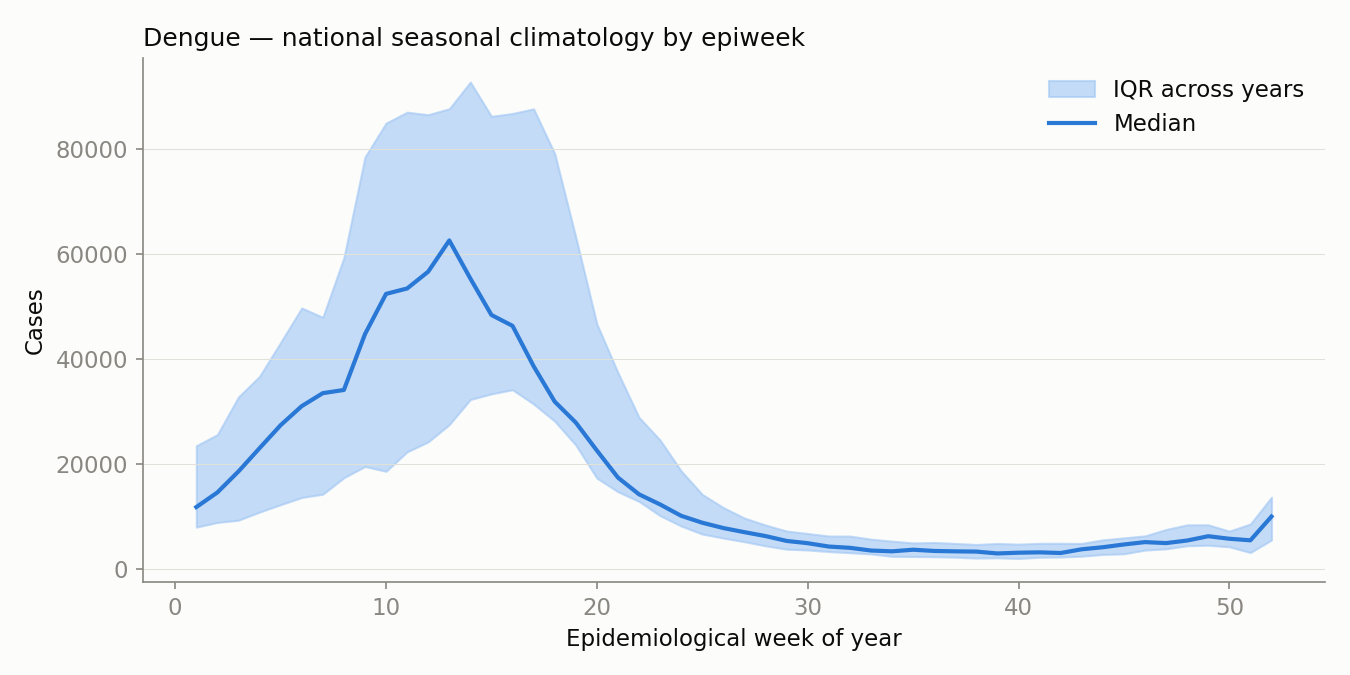
\includegraphics[width=0.8\textwidth]{../results/figures/dengue_climatology.png}
\caption{\textbf{S1 Fig. Seasonal climatology of dengue incidence by state.}}
\end{figure}

\begin{figure}[t]\centering
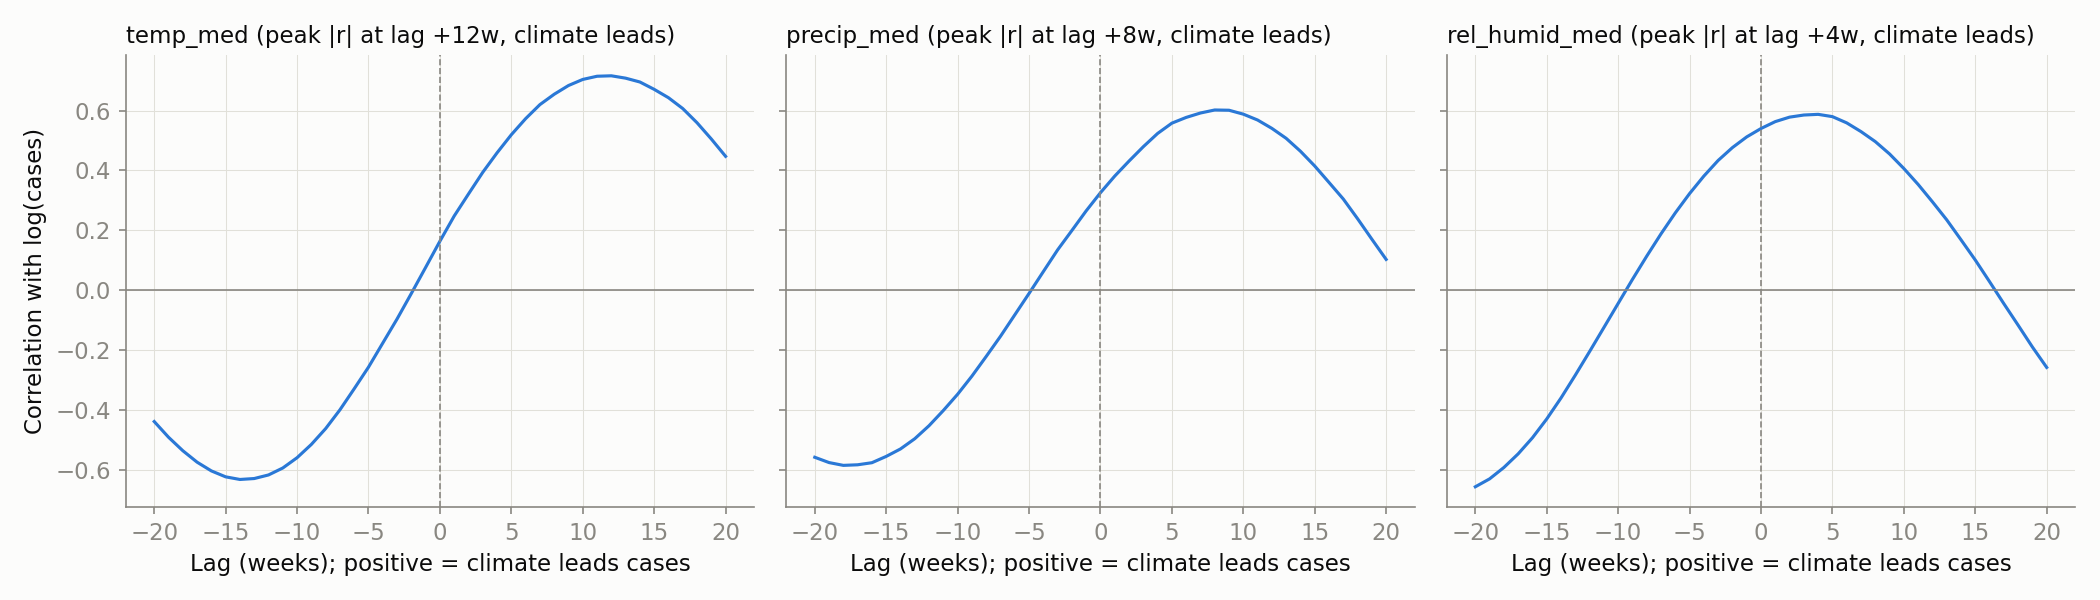
\includegraphics[width=0.8\textwidth]{../results/figures/climate_lag_cross_correlation.png}
\caption{\textbf{S2 Fig. Lagged cross-correlation of climate variables with dengue incidence.}}
\end{figure}

\begin{figure}[t]\centering
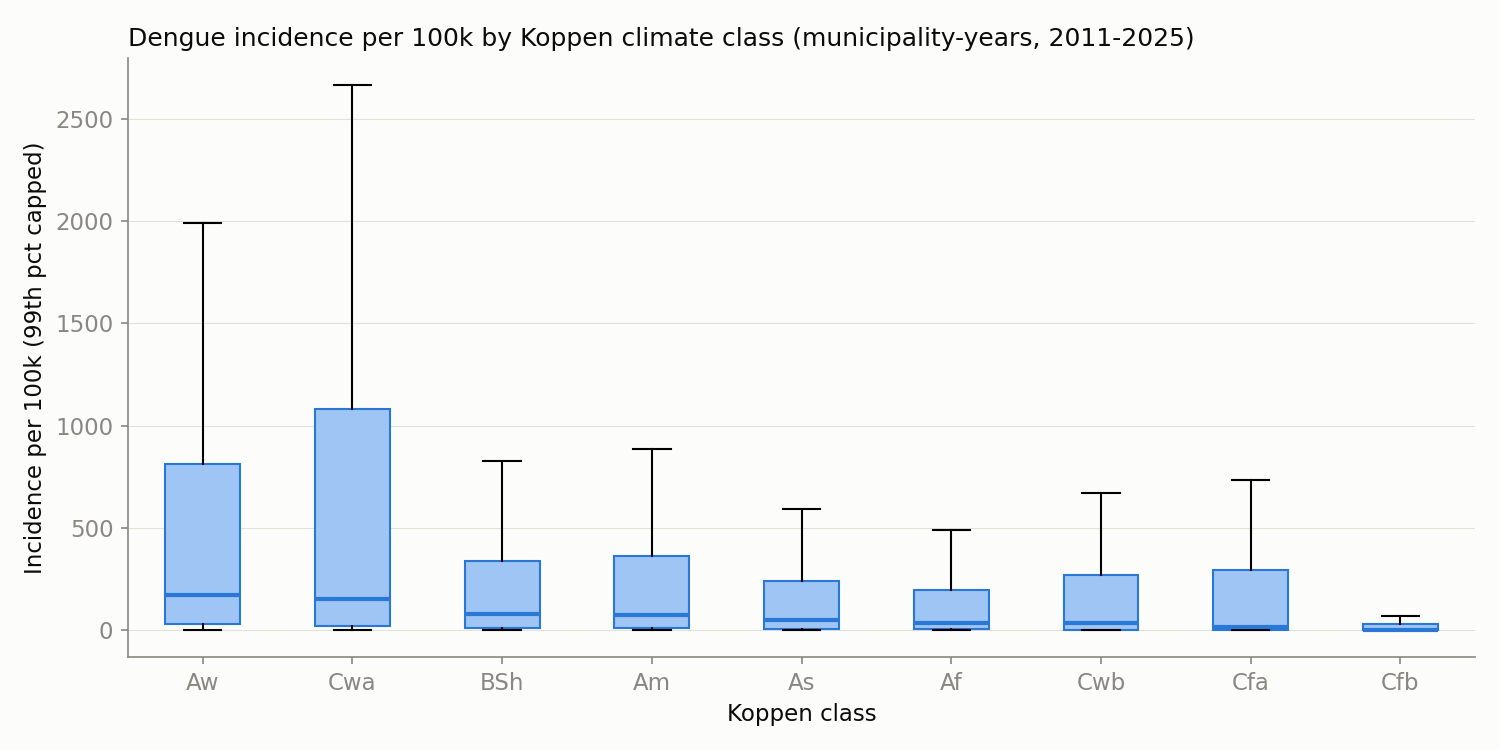
\includegraphics[width=0.75\textwidth]{../results/figures/dengue_incidence_by_koppen.png}
\caption{\textbf{S3 Fig. Dengue incidence by K\"oppen climate zone.}}
\end{figure}

\begin{figure}[t]\centering
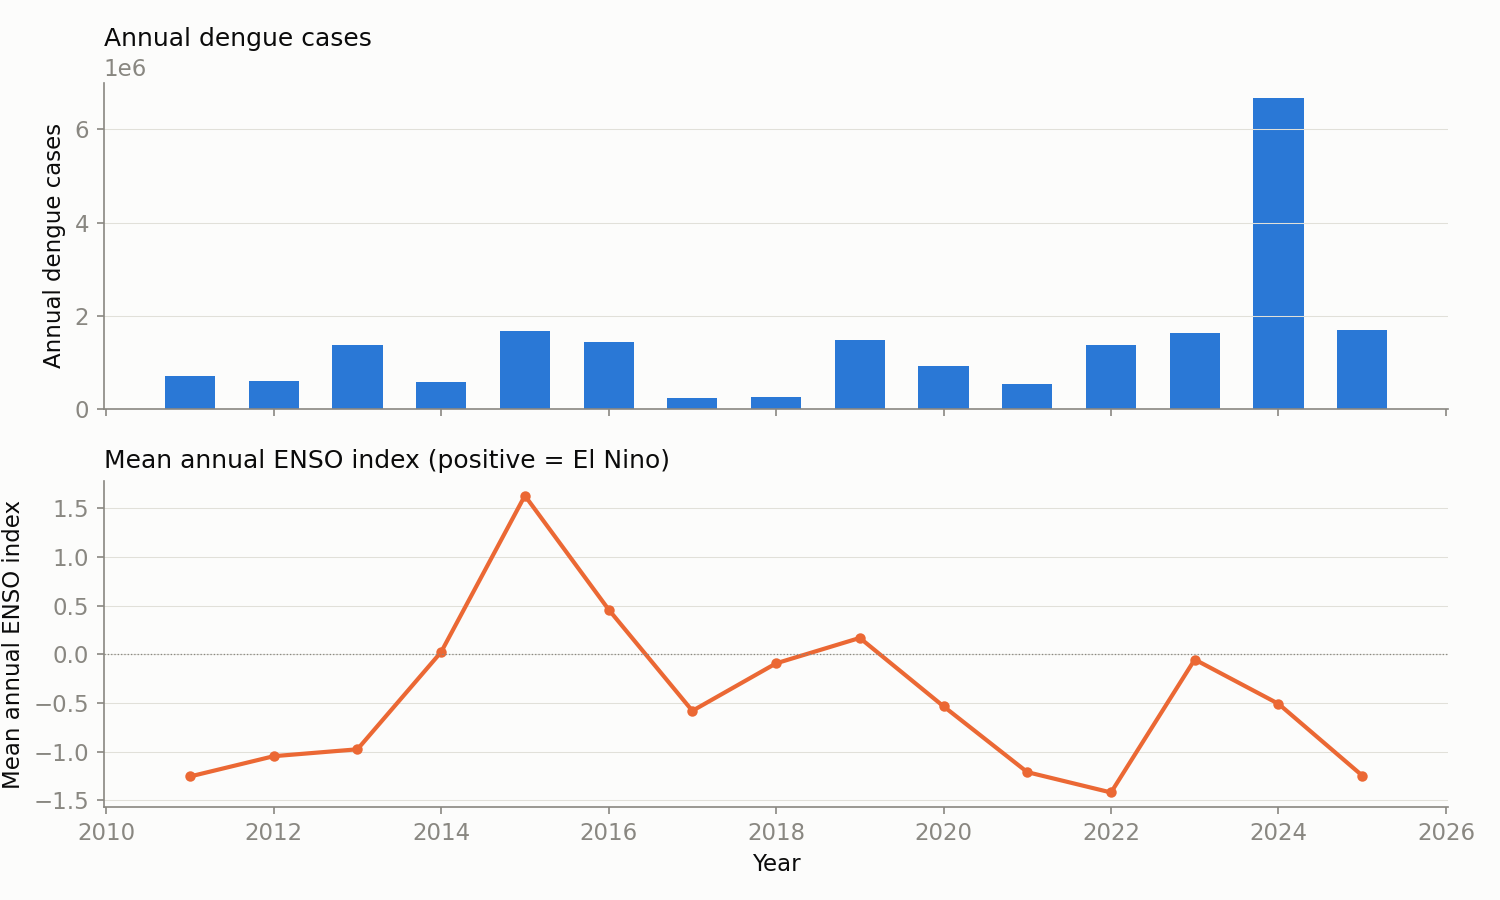
\includegraphics[width=0.75\textwidth]{../results/figures/dengue_vs_enso_annual.png}
\caption{\textbf{S4 Fig. Annual dengue totals versus the El Ni\~no--Southern Oscillation index.}}
\end{figure}

\begin{figure}[t]\centering
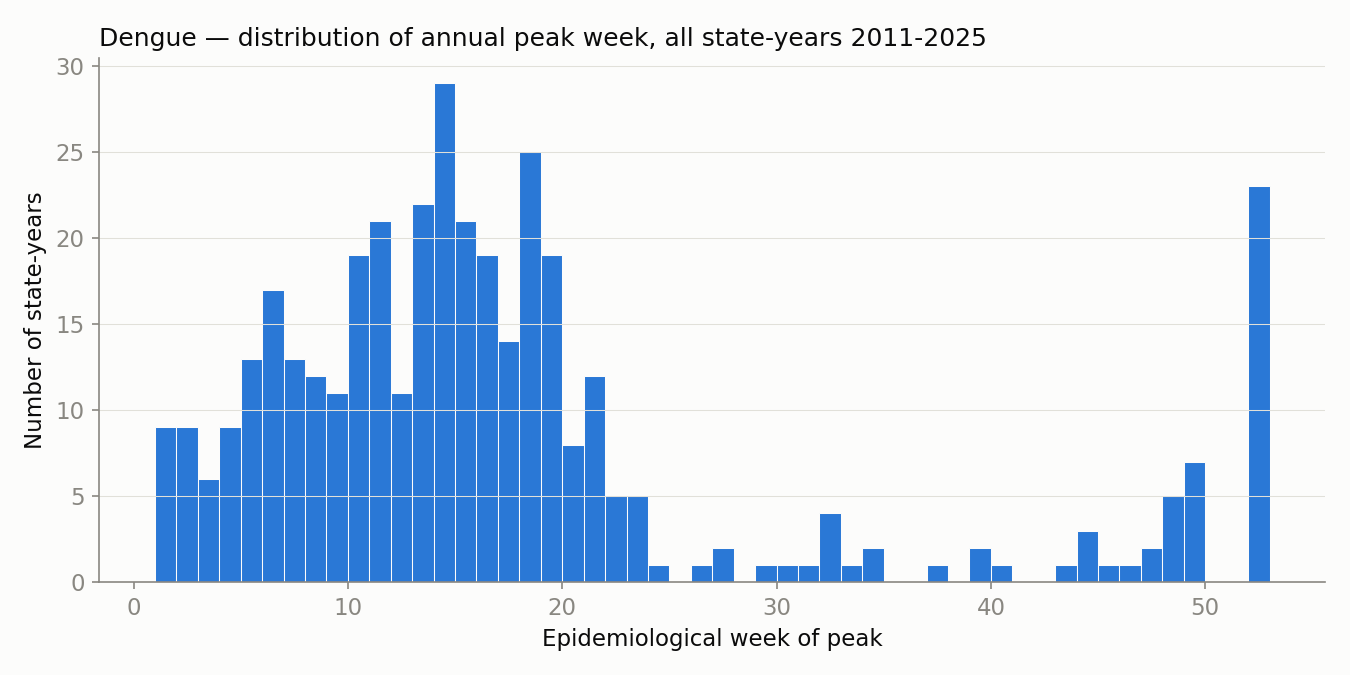
\includegraphics[width=0.75\textwidth]{../results/figures/dengue_peak_week_distribution.png}
\caption{\textbf{S5 Fig. Distribution of epidemic peak weeks across states and seasons.}}
\end{figure}

\section*{S7 Text. Reproducibility and provenance}
The complete pipeline is released as an installable package with a single command to reproduce every
result. Leakage safety, scoring correctness, model persistence, and every model family are covered by
an automated test suite that runs in continuous integration. All model fitting is deterministic under a
fixed seed: LightGBM uses its own deterministic mode, XGBoost and the mechanistic model fix their own
seeds, and the deep ensemble fixes the seed of
each member. A provenance manifest records the exact data checksums and code revision behind each
reported number, and the per-state scored predictions for all models are released so that any table or
figure can be regenerated. Validated submission files for the four official tracks (dengue and
chikungunya, at state and city level) are included.

\section*{S8 Text. Per-state model performance heatmap}
Table-based per-state comparisons do not scale to six models across 26 states. Fig~S6 gives the
same comparison as a heatmap: each cell is one model's mean log relative WIS against the
seasonal-naive baseline in one state, averaged over the four seasons, the same quantity underlying
the stability figure in the main text (Fig 3) but broken out by state instead of collapsed to a
mean and standard deviation. Green cells are better than the baseline and red cells are worse. Two
patterns are visible beyond the aggregate numbers already reported: the deep network's advantage is
concentrated in a subset of states (Ceara and Roraima most strongly) rather than uniform, and
the gradient-boosted model (XGBoost) is the only one of the six with states that are red, meaning
worse than
the seasonal-naive baseline (Sergipe most strongly, followed by Para\'iba, Amap\'a, Maranh\~ao, Par\'a,
Piau\'i, and Rond\^onia), which the state-level aggregate in
Table 1 does not show.

\begin{figure}[t]\centering
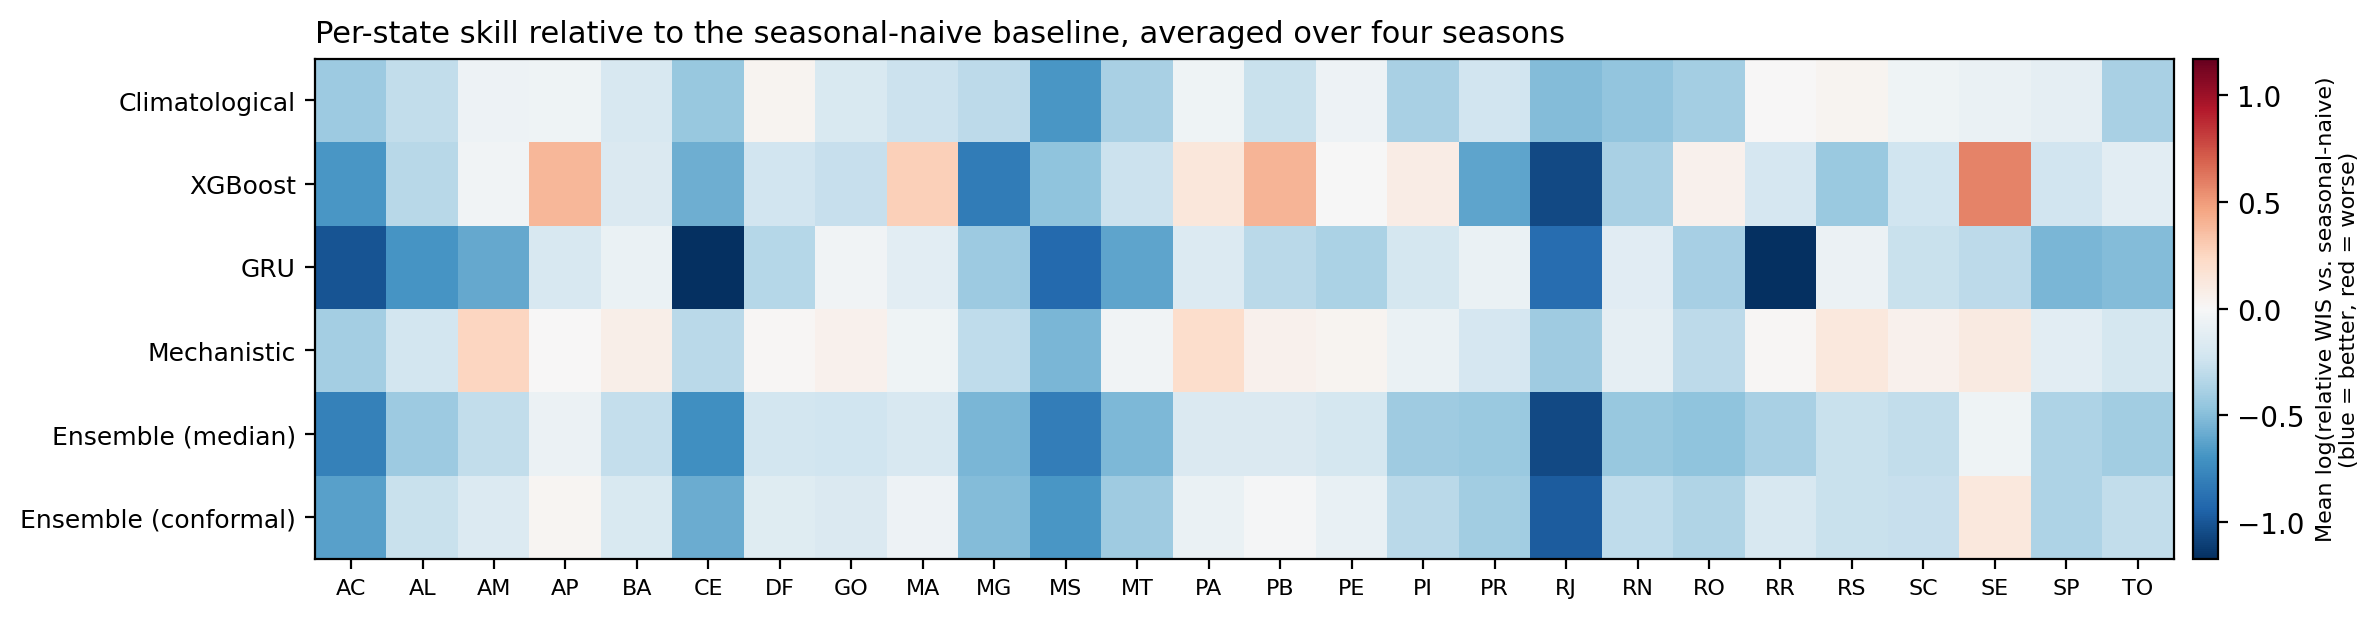
\includegraphics[width=\textwidth]{../results/figures/paper_state_heatmap.png}
\caption{\textbf{S6 Fig. Per-state skill relative to the seasonal-naive baseline.} Mean log
relative WIS by model and state, averaged over the four seasons. Green is better than baseline, red
is worse.}
\end{figure}

\section*{S9 Text. Calibration by percentile of the predictive distribution}
The reliability curve in the main text (Fig 8, Calibration and its correction) summarizes
calibration at four interval levels.
Fig~S7 shows where in the predictive distribution the miscalibration sits, using the probability
integral transform (PIT): a calibrated forecast places the observation uniformly across its own
distribution, so each of the ten bins cut by the nine submitted quantiles should hold its nominal
share. Two implementation details matter for quantile-reported count data. The ten bins have
unequal widths (25 percentage points at the centre, 2.5 at the tails), so raw counts would make
the central bins look over-full by construction; every panel therefore plots the ratio of observed
to expected share, where 1.0 is calibrated at any bin width. Case counts are also discrete and
often tie against their own predicted quantiles, so we use the non-randomized PIT for discrete
data: an observation tied against $k$ quantiles contributes $1/(k+1)$ to each bin it could occupy,
which is deterministic and reproducible, unlike the randomized alternative.

Three features are visible that the four-level reliability curve cannot show. First, the deep
network's overconfidence is symmetric and severe: both tail bins are over-full (3.5 and 9.6 times
their nominal share) while the central half is at roughly half its share, the signature of
intervals that are uniformly too narrow rather than merely mis-centred. Second, every model,
including the well-calibrated gradient-boosted one, carries an excess in the topmost bin. That
excess is the same under-prediction the WIS decomposition attributes to the 2024 season (main
text, Fig 9B), seen here as a distributional rather than a seasonal statement: the observation
lands above the 97.5th percentile far more often than it should, and no model family avoids this.
Third, conformal recalibration cuts the ensemble's topmost-bin excess from 4.4 to 2.4 times
nominal while leaving the rest of the distribution close to flat, which is the intended asymmetric
effect stated in the main text made visible bin by bin.

The mechanistic model and the recalibrated ensemble show near-empty lowest bins (ratios of 0.01
and 0.00). This is an expected consequence of non-negativity rather than a defect: their lower
quantiles are clipped at zero, an observation of zero then ties against them, and the
non-randomized PIT spreads that tie across the bins it could occupy instead of charging it to the
bottom bin. Widening intervals downward cannot help a count that is already at its floor.

\begin{figure}[t]\centering
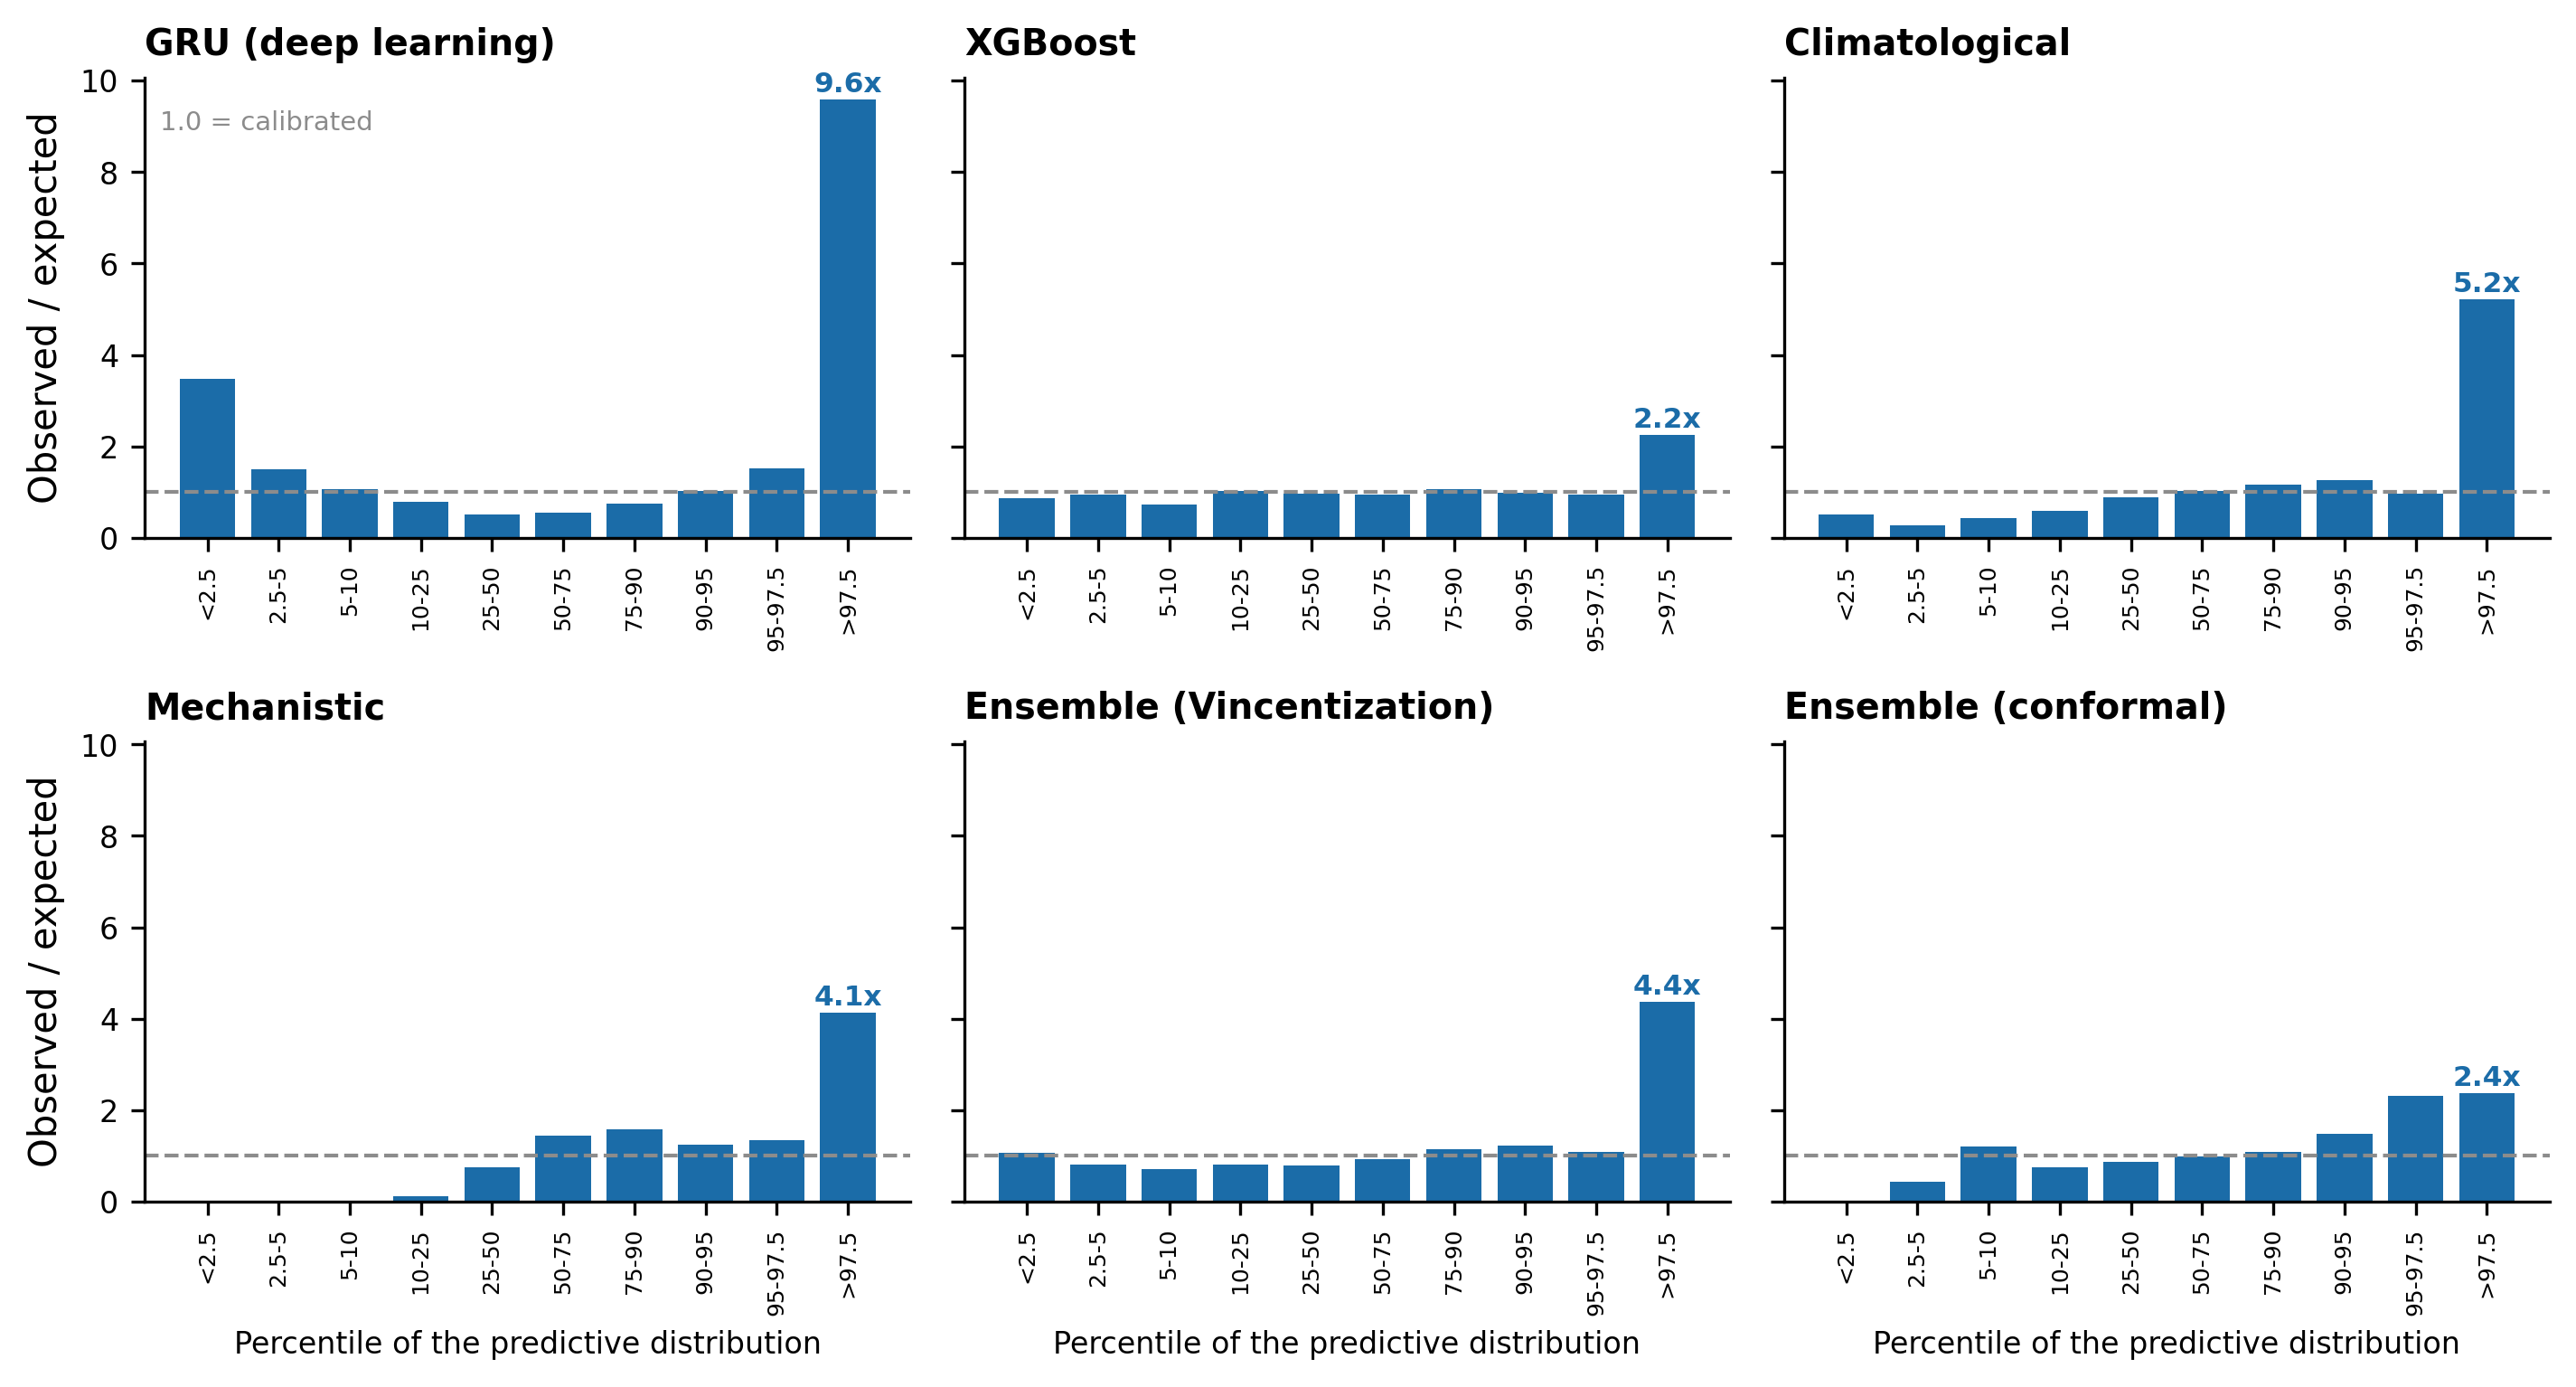
\includegraphics[width=\textwidth]{../results/figures/paper_pit.png}
\caption{\textbf{S7 Fig. PIT calibration by model.} Ratio of observed to expected share in each of
the ten bins cut by the nine submitted quantile levels, so 1.0 (dashed line) is calibrated at any
bin width. A U shape indicates intervals that are too narrow, a central hump intervals that are
too wide, and a tilt indicates bias. The tallest bar in each panel is labelled, since the shared
vertical scale is set by the deep network's outlier. Computed on all four seasons and 26 states.}
\end{figure}

\section*{S10 Text. Glossary}
Terms used throughout the main text and this document, in order of first appearance.

\begin{itemize}
\item \textbf{WIS (weighted interval score)}:the challenge's scoring rule for a probabilistic
forecast; combines median accuracy with interval width and coverage into one number, lower is
better (S1 Text gives the formula and a worked example).
\item \textbf{Coverage (nominal vs.\ empirical)}:nominal coverage is an interval's stated
probability (e.g.\ 90 percent for the 90 percent interval); empirical coverage is the fraction of
observations it actually contained. A well-calibrated model has the two close together.
\item \textbf{Sharpness}:how narrow, and therefore informative, a model's prediction intervals
are, independent of whether they are well calibrated.
\item \textbf{Dispersion, under-prediction, over-prediction (WIS components)}:the three
non-negative pieces WIS decomposes into: dispersion is the interval-width penalty present even for
a perfectly centered forecast; the other two are penalties for the observation falling above or
below the stated interval.
\item \textbf{Relative WIS}:one model's WIS divided by a baseline model's WIS on the same
forecasting units, a pairwise comparison (Cramer et al.\ 2022) that removes shared, unit-level
variance; we report its logarithm so a model twice as good and twice as bad are symmetric.
\item \textbf{Normalized WIS}:the sum of WIS divided by the sum of observed cases; scale-free
across states/cities of very different size, and the challenge's own headline metric.
\item \textbf{Vincentization}:combining several models' forecasts by taking, at every quantile
level separately, the median of the models' values at that level.
\item \textbf{Conformalized quantile regression (CQR)}:calibrating one model's own quantile
predictions, during fitting, by measuring on held-out data how much each quantile needs to shift to
reach its nominal coverage.
\item \textbf{Conformal recalibration (this paper's ensemble-level step)}:a separate,
after-the-fact widening of the already-combined ensemble's intervals, by a multiplicative factor per
interval level tuned on one season and reused unchanged thereafter; distinct from CQR, which
calibrates one model during fitting rather than the combined ensemble afterward.
\item \textbf{Synthetic-origin panel}:the training set built for XGBoost/LightGBM/GRU: every historical
week within a fold's cutoff-filtered history becomes a candidate forecast origin, crossed with
horizons 1--67 weeks ahead, so a handful of true evaluation windows becomes tens of thousands of
training rows.
\item \textbf{Block bootstrap}:a resampling technique that repeatedly draws whole state-season
units (not individual weeks) with replacement to estimate how much a summary statistic (e.g.\
normalized WIS) would vary under the data's actual dependence structure.
\item \textbf{Paired comparison}:comparing two models' scores on the exact same forecasting units
and looking at the difference, rather than comparing their two separate score distributions; cancels
variance that is common to both models (e.g.\ from an unusually hard season).
\item \textbf{Negative-binomial (head/distribution)}:a count-data distribution more flexible than
Poisson, allowing variance to exceed the mean, as case-count data typically do; the GRU's output
layer and the mechanistic model's observation model both use it.
\item \textbf{Richards curve}:a flexible, S-shaped growth-then-plateau curve classically used to
summarize an epidemic's rise and fall over a season; the mechanistic model fits one per historical
season and resamples from these fits to build future trajectories.
\item \textbf{Distributed-lag non-linear model (DLNM)}:a modeling structure that lets a
covariate's effect on the outcome be both delayed (this week's climate affecting cases several
weeks later) and non-linear in the covariate's own value.
\item \textbf{Empirical-Bayes pooling (shrinkage)}:partially pulling each unit's (e.g.\ each
state's) own estimate toward a shared average across a group of units, to borrow statistical
strength when individual units are noisy.
\item \textbf{Onset week, peak week/magnitude, total cases (operational summaries)}:decision-relevant
quantities WIS does not directly show: the first week a series reaches a fraction of its own peak;
the timing and size of the true peak week; and the season's total case count; each reported as an
error relative to the true value (Results Section~2.11 of the main text).
\end{itemize}

\end{document}
